\part{Service-to-Service Communication}

\begin{frame}[fragile]{Simple Service Call (Synchronous)}
Create REST requests using \colorlink{http://docs.spring.io/spring-framework/docs/current/javadoc-api/org/springframework/web/client/RestTemplate.html}{\codealt{RestTemplate}} for client-side HTTP access
\begin{block}{Call Service}
\begin{lstlisting}
@Value("${URL}") //e.g. "http://example.org/api/v1.0/users/"
String url;

@Inject
private final RestTemplate restTemplate;

public User callGetUserService() {
    try {
        ResponseEntity<User> response = restTemplate.getForEntity(url, User.class);
    } catch(HttpStatusCodeException error) {
        logger.error("received HTTP status code: {}", error.getStatusCode());
        throw error;
    }
    return response.getBody();
}
\end{lstlisting}
\end{block}
\end{frame}



\begin{frame}{Exercises: 16}
\begin{figure}
	\includeGraphicsExerciseSixteen{width=\textwidth}
	\end{figure}
 \colorlink{https://github.com/ccjavadev/cc-coursematerial/blob/master/Service2ServiceCommunication/Exercise_16_Call_UserService.md}{Exercise 16: Call User Service}
\end{frame}

\begin{frame}{Challenges}
\begin{columns}[T] 
\begin{column}{.67\textwidth}
Service dependencies introduce latency and other points of failure
\begin{itemize}
	\item What if called service does not answer \\(in time)?
	\item How to avoid cascading failures / latency?
	\item How to avoid flooding server after restart?
 \end{itemize}
\end{column}
\hfill
\begin{column}{.29\textwidth}
\centerline{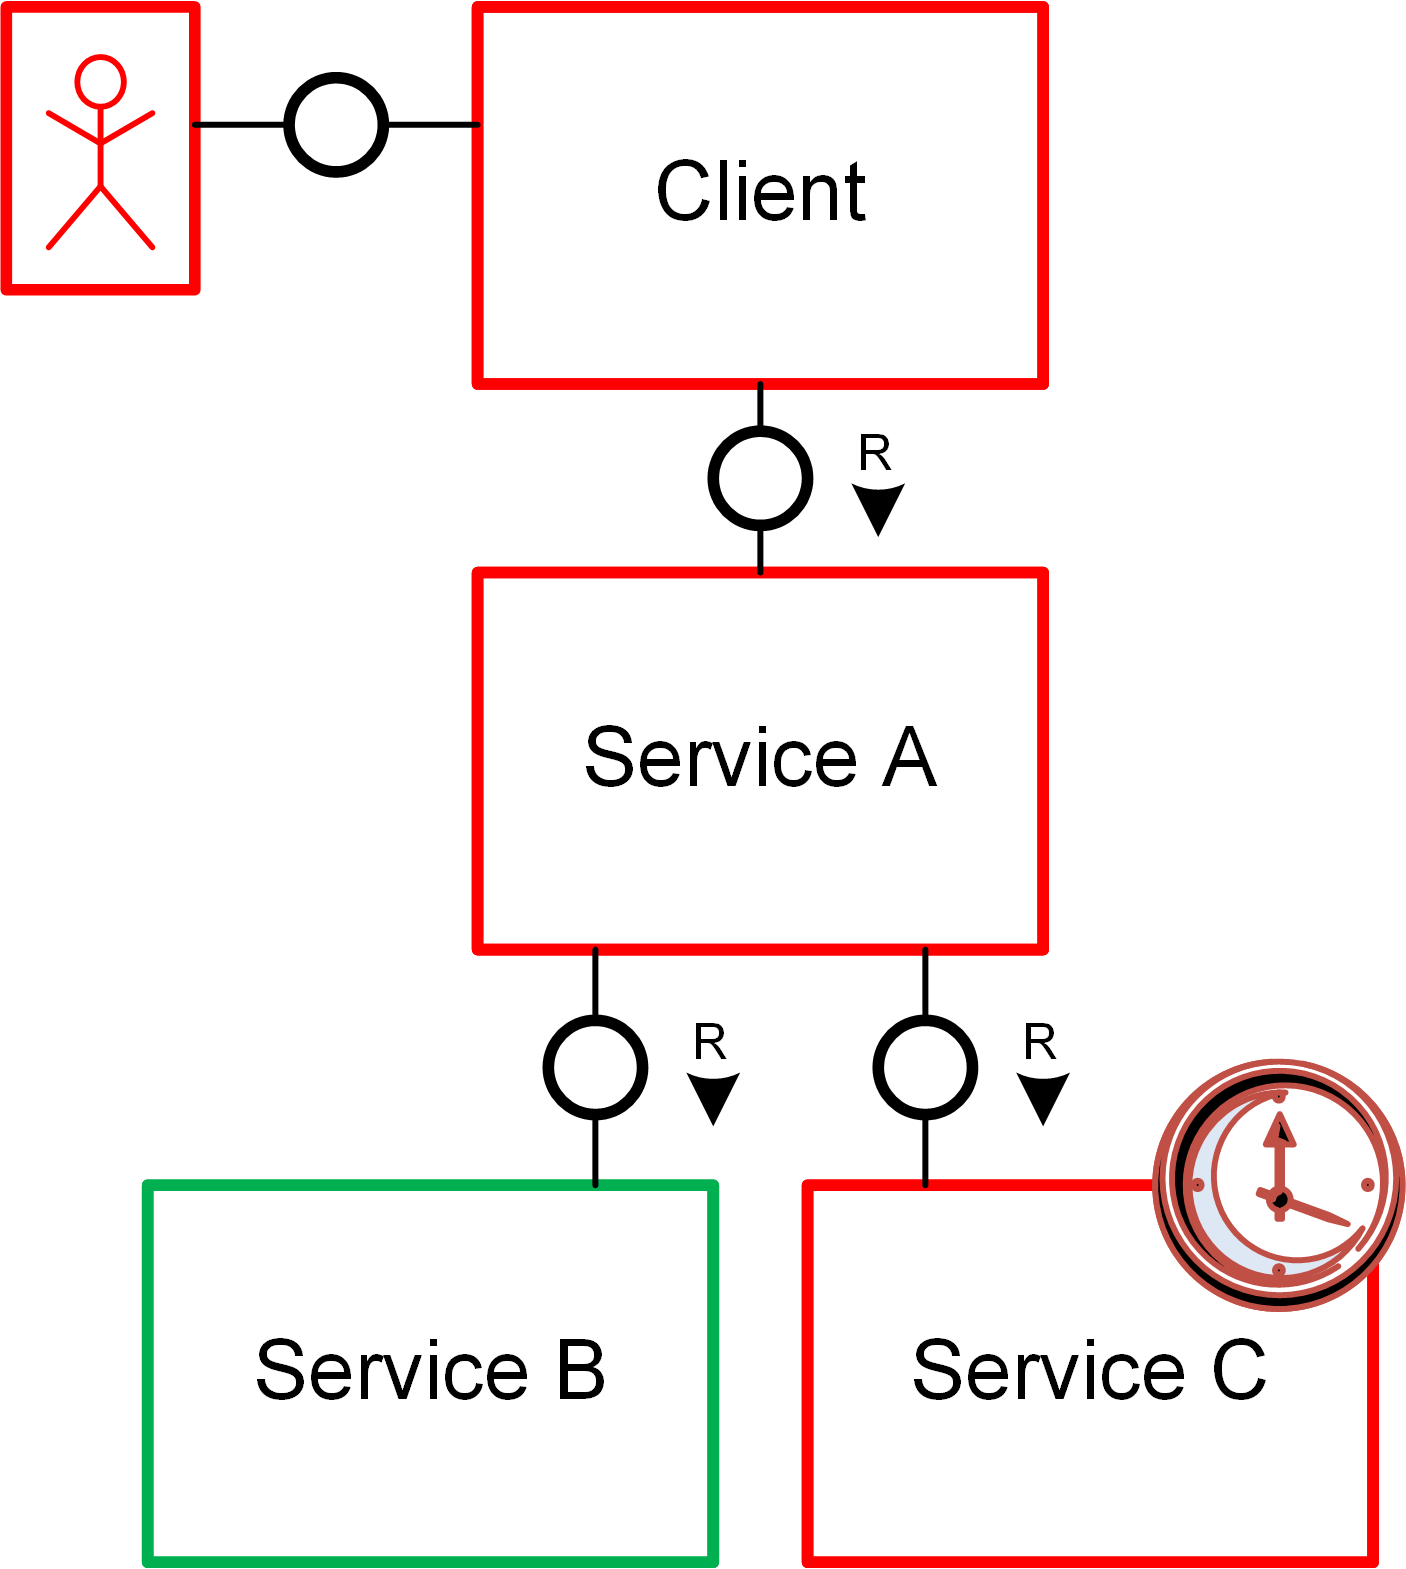
\includegraphics[width=\textwidth]{../Service2ServiceCommunication/images/CascadingIssue}}
\end{column}
\end{columns}

\vfill
\visible<2->{
\begin{block}{A Typical Problem Case}
Customer creates an order. This triggers the order creation and if it is successful, the warehouse system is informed for dispatching the order.
\\\vspace{2mm}
But - what should happen if the call to the warehouse system fails?
\end{block}
}
\end{frame}

\begin{frame}{Resilience}
\textbf{Definition of resilience:}
\newline
the ability of a system to handle unexpected situations 
\begin{itemize}
	\item without the user noticing it (best case)
	\item with a graceful degradation of service (worst case)
\end{itemize}
\vfill
\visible<2->{
\textbf{Fallback approach for graceful degradation}
\\what result to use if the call fails
\begin{itemize}
	\item use cached (potentially outdated) value 
	\item use sensible default
	\item try second-best alternative (e.g. apply to message queue)
\end{itemize}
}
\end{frame}

\begin{frame}{Hystrix - Resilience Library}
%\textbf{A)} protect yourself from unhealthy services and \newline
%\textbf{B)} protect the downstream service from more calls that may be having an adverse impact

\begin{block}{Hystrix}
\vspace{-2mm}
\begin{itemize}
\item Easy to start with
\item Many fault-tolerance patterns implementable
	\begin{itemize}
	\item Fail fast / silent 
	\item Circuit breaker pattern
	\item Load shedding\footnote{Load shedding: requests are rejected under certain conditions} (thread pool)
	\item Advanced: Request caching
	\end{itemize}
\item Many configuration options
\end{itemize}
\vspace{-2mm}
\end{block}
\vspace{-2mm}
\colorlink{https://github.com/Netflix/Hystrix/wiki}{Hystrix Wiki}

\end{frame}

\begin{frame}[fragile]{Hystrix Command}
Wrap all potentially failing calls in a \codealt{HystrixCommand}
\begin{lstlisting}
public class MyCommand extends HystrixCommand<String> {
    public MyCommand() {
        super(HystrixCommandGroupKey.Factory.asKey("ExampleGroup"));
    }

    @Override
    protected String run() {
        // creates client, sends request, handles response
        return callGetUserService(id);
    }
}
\end{lstlisting}
\vfill
\footnotesize{Note: Each \codealt{HystrixCommand} is executed within a separate thread and is timed out automatically after 1000ms by default.}
\end{frame}


   
\begin{frame}[fragile]{Hystrix Command - Execution Patterns}

Synchronous execution
\begin{lstlisting}
String string = new MyCommand().execute();
\end{lstlisting}

\begin{visibleenv}<2->
Asynchronous execution
\begin{lstlisting}
Future<String> future = new MyCommand().queue();
String string = future.get(); // this blocks, consider future.isDone()
\end{lstlisting}
\end{visibleenv}

\begin{visibleenv}<3->
Reactive execution - inverts control flow (IoC) \\mechanism to process data streams\footnote{advanced topic: out of scope for this course}
\begin{lstlisting}
Observable<String> observable = new MyCommand().observe();
observable.subscribe(new Observer<String>() {
        public void onError(Throwable e) { /* observed call encounters issue */ }

        public void onNext(String v) { /* observed call emits data */ }
        
        public void onCompleted() { /* after the last onNext() call */ }
});
\end{lstlisting}
\end{visibleenv}
\end{frame}

\begin{frame}{Exercises: 17}
	\begin{figure}
		\includeGraphicsExerciseSeventeen{height=0.6\textheight}
	\end{figure}
 	\colorlink{https://github.com/ccjavadev/cc-coursematerial/blob/master/Service2ServiceCommunication/Exercise_17_Introduce_Hystrix.md}{Exercise 17: Introduce Hystrix}
\end{frame}

\begin{frame}{Hystrix Flowchart}
\centerline{
	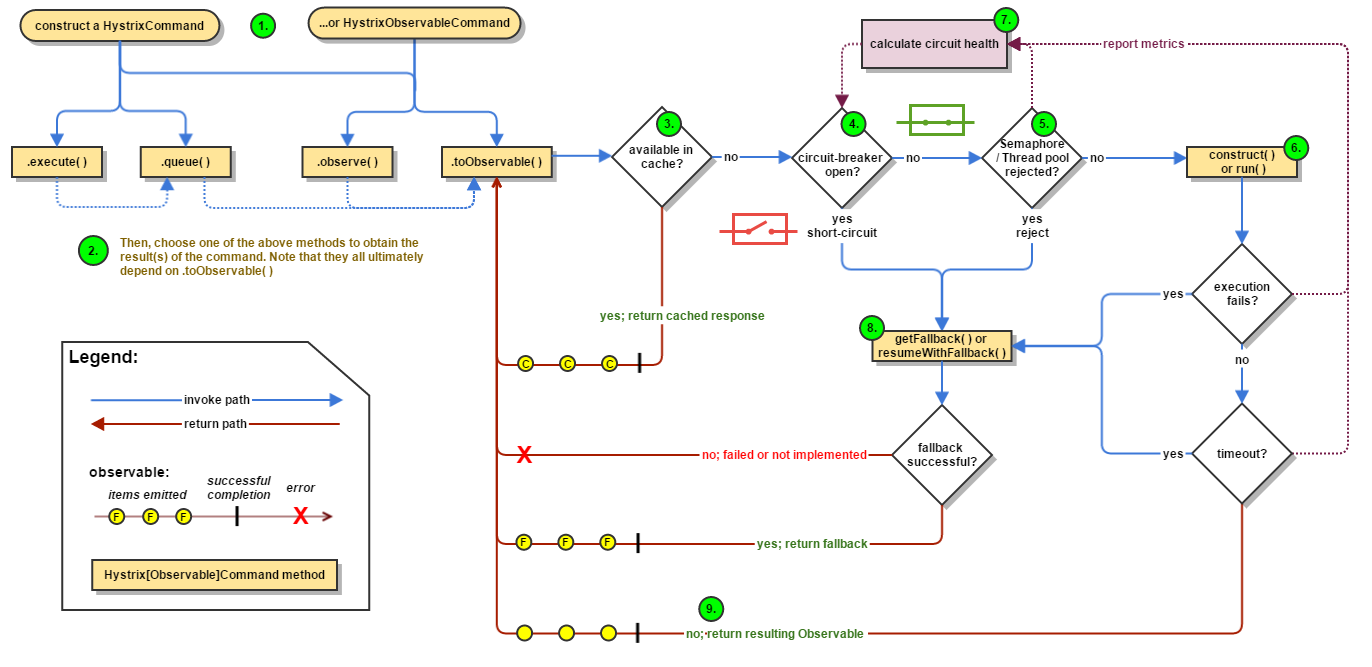
\includegraphics[width=\paperwidth]{../Service2ServiceCommunication/images/hystrix-flow-chart-original}
}
\colorlink{https://github.com/Netflix/Hystrix/wiki/How-it-Works}{Hystrix Wiki: How it works}
\end{frame}

\begin{frame}[fragile]{Hystrix Fallback}
\begin{lstlisting}
public class MyCommand extends HystrixCommand<String> {
	...
	
    @Override
    protected String getFallback() {
        if (isResponseTimedOut()) {
            logger.warn("execution timed out");
        }
        if (isFailedExecution()) {
            logger.error("execution failed: {}", getFailedExecutionException().getMessage());
        }
        return "fallback value";
    }
}
\end{lstlisting}
\footnotesize{Note: Fallback logic is performed when a request fails, times out, or is rejected (thread pool is full).}
\end{frame}

\begin{frame}[fragile]{Hystrix Configuration - Some Examples}
\begin{itemize}
\scriptsize
\item \codealt{hystrix.\textbf{threadpool.default.coreSize}}
\\Maximum number of concurrently executed threads per Command (Group) (default: 10)
\item \codealt{hystrix.command.\textcolor{red}{*}.execution.isolation.\textbf{thread.timeoutInMilliseconds}}
\\Time to wait for the \codealt{run()} method to complete (default: 1000)
\item \codealt{hystrix.command.\textcolor{red}{*}.\textbf{circuitBreaker.errorThresholdPercentage}}
\\Error percentage at which breaker trips open (default: 50)
\item \codealt{hystrix.command.\textcolor{red}{*}.\textbf{circuitBreaker.sleepWindowInMilliseconds}}
\\Timeframe in which requests are rejected, after tripping the circuit, and before reattempting to use the resource by permitting single requests to pass through(default: 5000)
\end{itemize}
\footnotesize{\textcolor{red}{*} must be replaced by \codealt{default} or any \codealt{CommandKey}}
\vfill
\colorlink{https://github.com/Netflix/Hystrix/wiki/Configuration}{Hystrix Configuration}
\end{frame}

\begin{frame}[fragile]{Hystrix Configuration - Keys Explained}
\begin{columns}[T] 
\begin{column}{.5\textwidth}
\only<1>{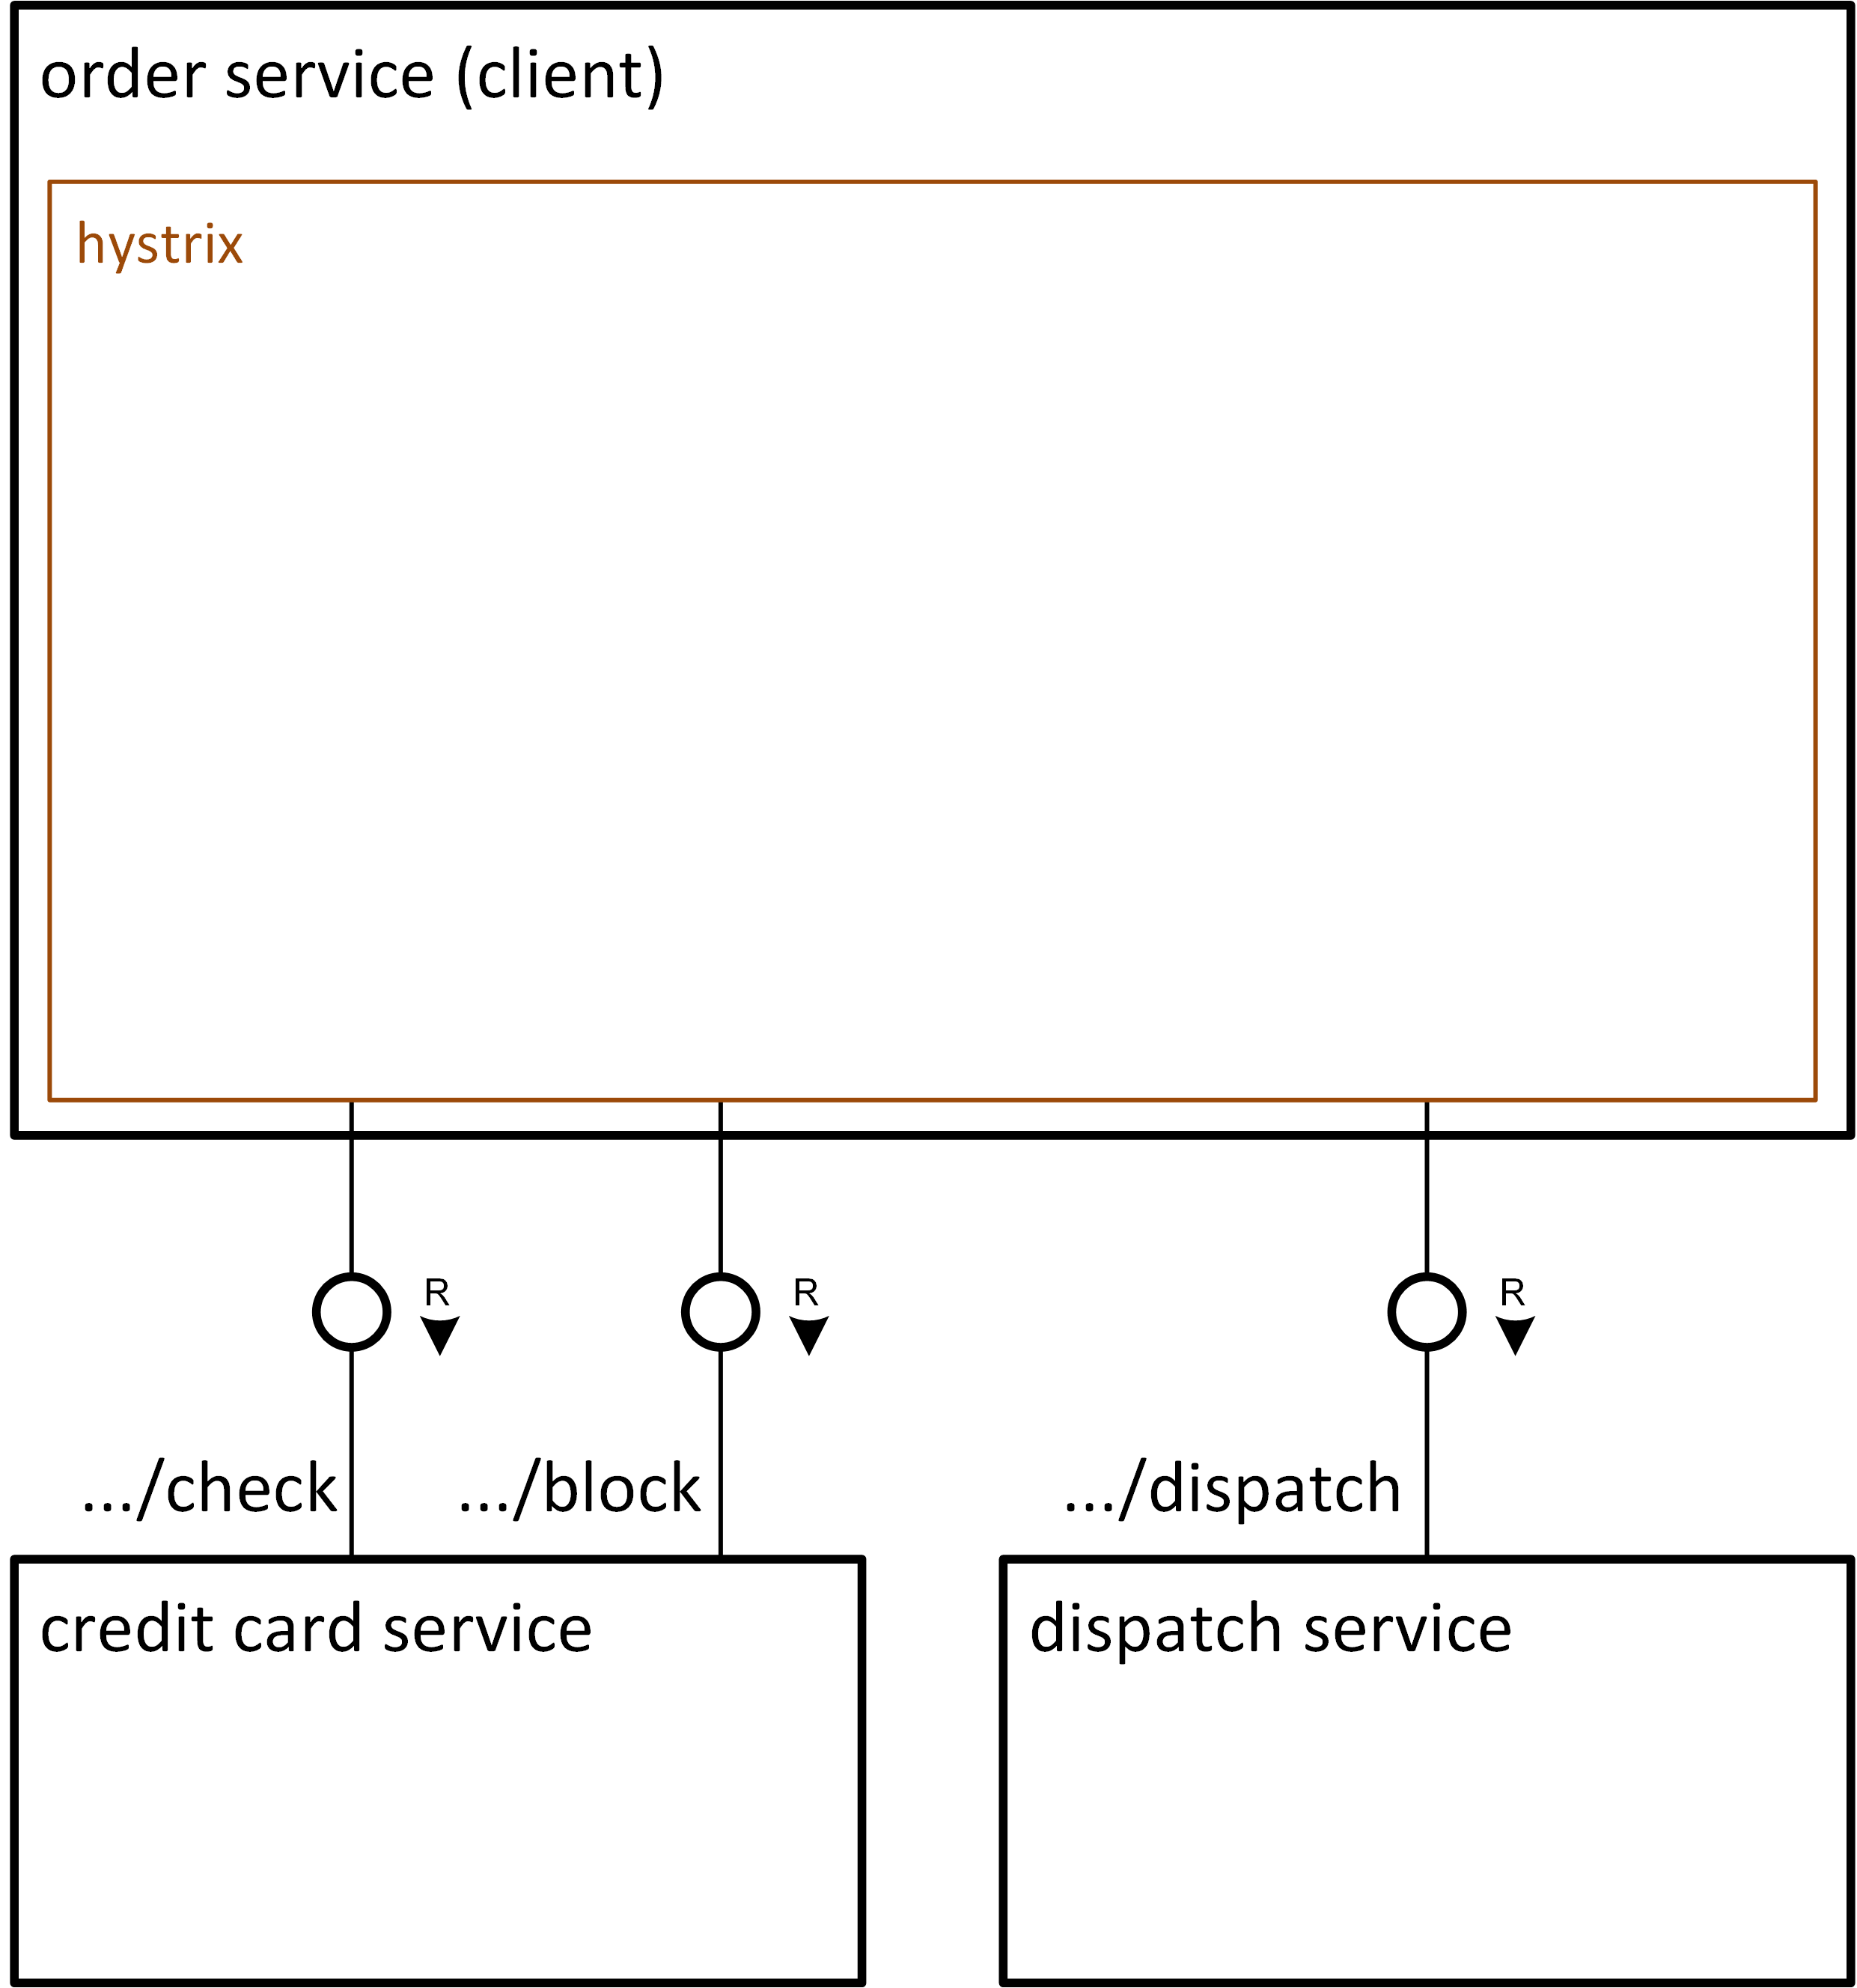
\includegraphics[height=0.6\textheight]{../Service2ServiceCommunication/images/Hystrix_Insights_1}}
\only<2,3>{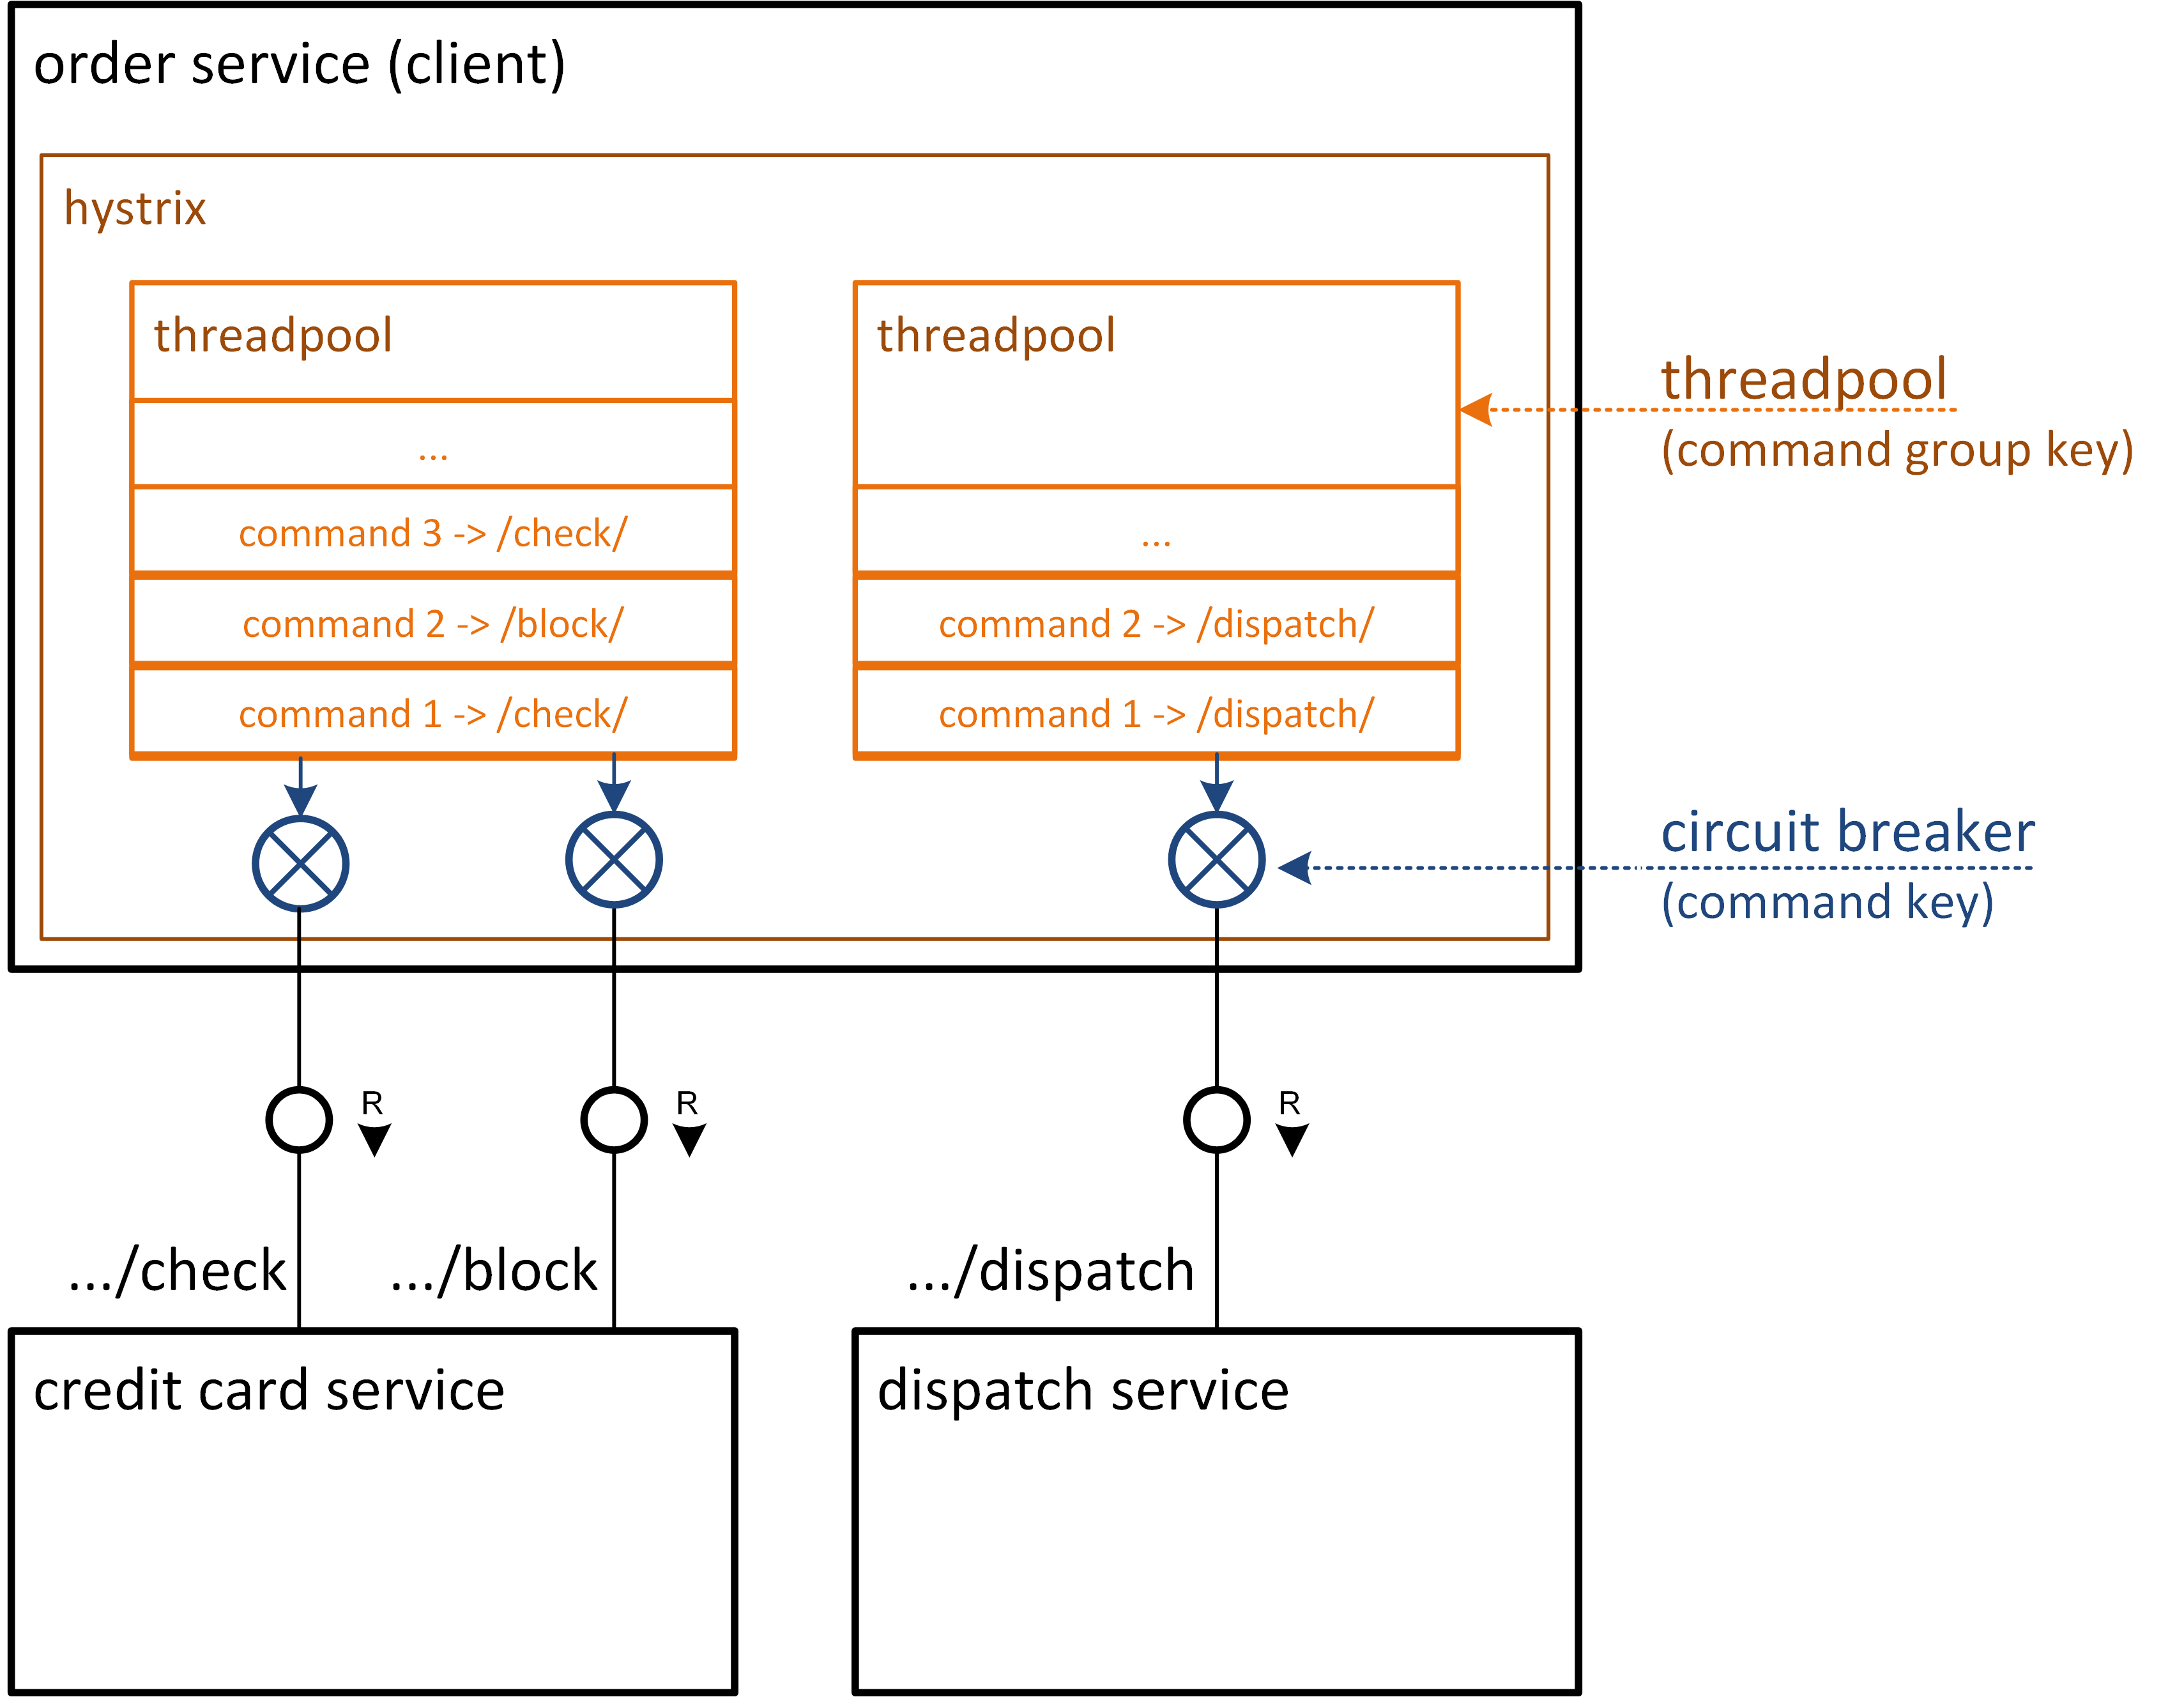
\includegraphics[height=0.6\textheight]{../Service2ServiceCommunication/images/Hystrix_Insights_2}}
\end{column}
\hfill
\begin{column}{.46\textwidth}
\only<3>{
\small
\begin{itemize}
\item define \codealt{CommandGroupKey} per service name e.g. "CreditCard" 
\item define \codealt{CommandKey} per \\logical operation name \\e.g. "CreditCard.BlockAmount" 
\end{itemize}
}
\end{column}
\end{columns}


\end{frame}

\begin{frame}{Exercise 18}
	\begin{figure}
		\includeGraphicsExerciseEighteen{height=0.7\textheight}
	\end{figure}
	\colorlink{https://github.com/ccjavadev/cc-coursematerial/blob/master/Service2ServiceCommunication/Exercise_18_Make_Communication_Resilient.md}{Exercise 18: Make communication more resilient}
\end{frame}


\begin{frame}{[Optional] Exercise 19}
	\begin{figure}
		\includeGraphicsExerciseNineteen{height=0.6\textheight}
	\end{figure}
	\colorlink{https://github.com/ccjavadev/cc-coursematerial/blob/master/Service2ServiceCommunication/Exercise_19_Transfer_CorrelationID.md}{Exercise 19: Transfer Correlation-ID}
\end{frame}

\begin{frame}[fragile]{Service Composition Patterns}{Orchestration vs. Choreography}
\begin{columns}[T] 
\begin{column}{.48\textwidth}
\textbf{Orchestration (sync)}\\
\small
\vspace{-2mm}
\begin{itemize}
	\item Request \& response
	\item Caller calls dep. service directly
	\item Use when result is needed to complete operation
\end{itemize}
\vspace{3mm}
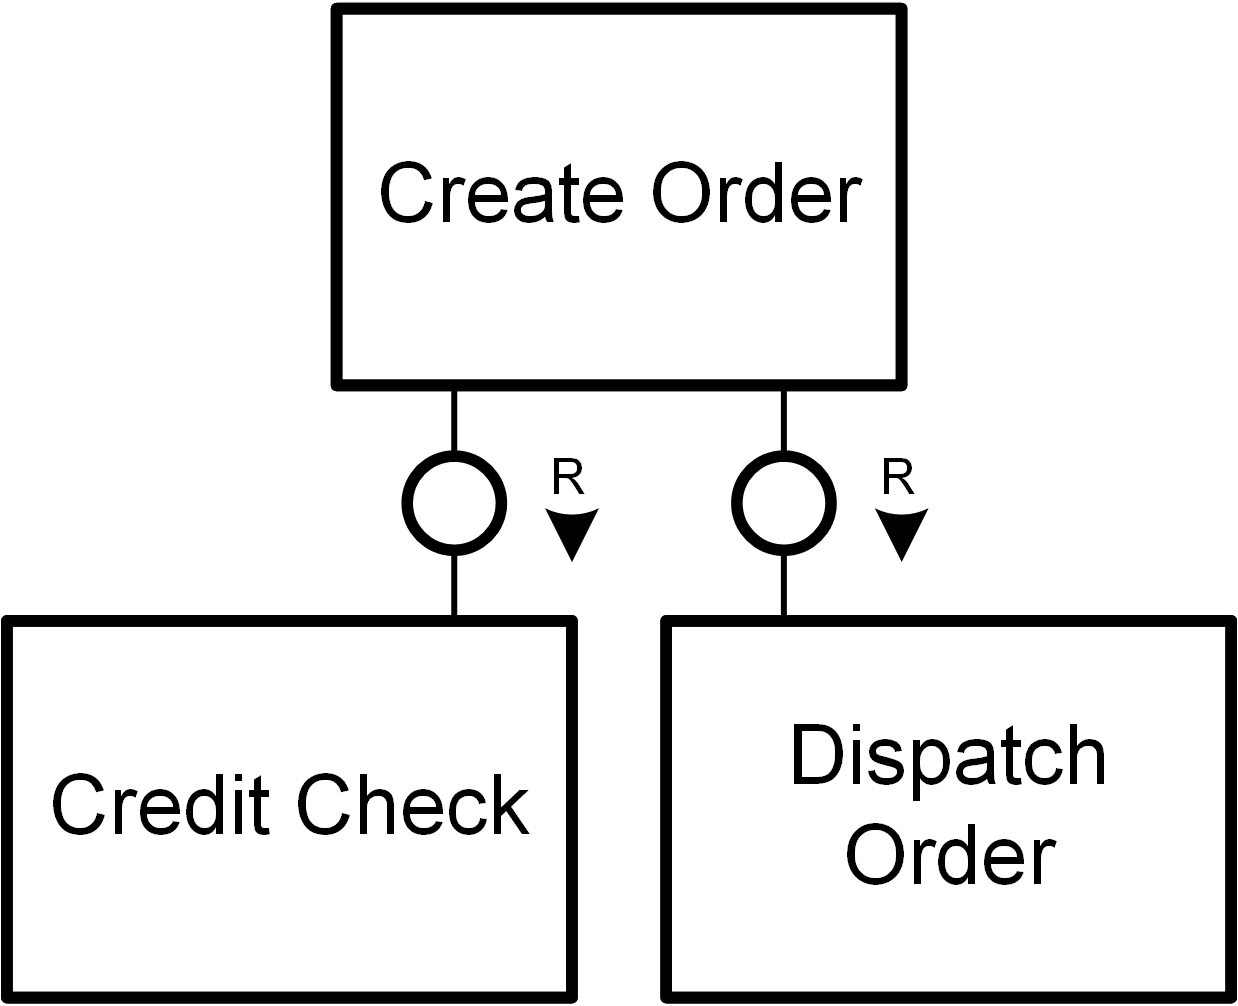
\includegraphics[height=0.25\textheight]{../Service2ServiceCommunication/images/Orchestration}
\end{column}
\hfill
\begin{column}{.48\textwidth}
\visible<2->{
\textbf{Choreography (async)}\\
\small
\vspace{-2mm}
\begin{itemize}
	\item Fire \& forget
	\item Caller publishes event
	\item Use when multiple consumers want to react asynchronously to events 
\end{itemize}
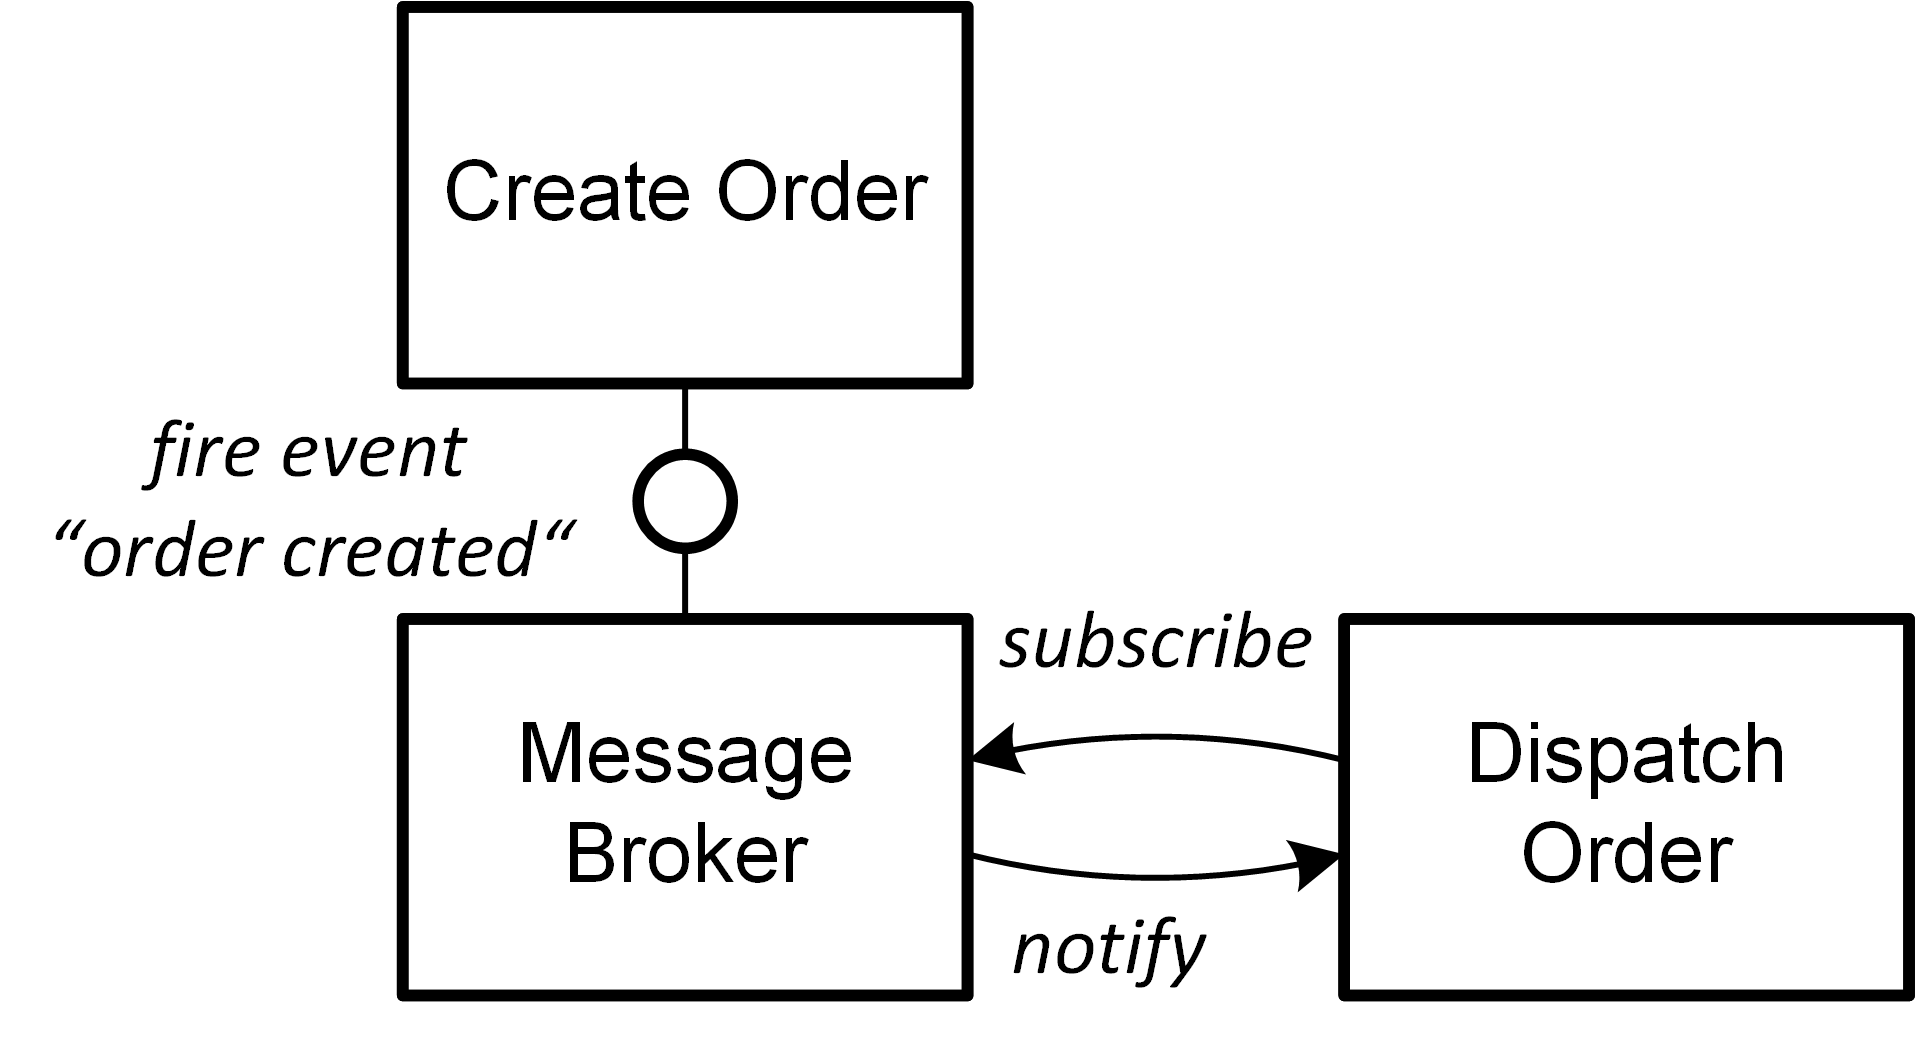
\includegraphics[height=0.25\textheight]{../Service2ServiceCommunication/images/Choreography}
}
\end{column}
\end{columns}
\vfill
\small
\visible<3->{
Message Brokers like \textbf{\codealt{RabbitMQ}} offer APIs to publish events and handle subscriptions allowing the consumers to be notified when an event arrives.
}
\end{frame}

\begin{frame}{RabbitMQ - Message Broker}
\textbf{Important to gain high performant and resilient cloud applications!}
\vfill 
Supports different Service Qualities as per AMQP message protocol
\begin{itemize}
\item \textit{fire-and-forget} (often non-durable)
\item \textit{at-least-once} and \textit{exactly-once} (message needs to be persisted till consumer sends acknowledgement back to RabbitMQ)
\end{itemize}
\vfill
\visible<2->{
Queues are bound to "Exchanges" to support these options
\begin{columns}[T] 
\begin{column}{.5\textwidth}
\begin{itemize}
\item direct binding using \textit{routing key}
\item routing by \textit{topic} e.g. "*.sap.*" 
\item broadcast message to multiple queues (\textit{fanout})
\end{itemize}
\end{column}
\begin{column}{.46\textwidth}
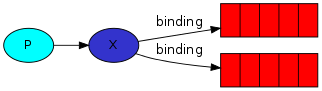
\includegraphics[width=\textwidth]{../Service2ServiceCommunication/images/RabbitMQ_Exchanges}
\end{column}
\end{columns}
\hfill
\colorlink{https://www.rabbitmq.com/getstarted.html}{RabbitMQ Tutorials}
}
\end{frame}

\begin{frame}[fragile]{Simple Message Broadcasting - Provider}
\small
\begin{block}{Setup using \codealt{AmqpAdmin}}
\begin{lstlisting}[language=Java,belowskip=-3mm,aboveskip=0mm]
public class MessageProvider {
   @Value("${ROUTING_KEY}") String routingKey;
    
   @Inject 
   public MessageProvider(AmqpAdmin amqpAdmin, RabbitTemplate rabbitTemplate) {
      amqpAdmin.declareQueue(new Queue(routingKey)); // creates queue, if not there
      this.rabbitTemplate = rabbitTemplate;
   }
   ...
}
\end{lstlisting}
\end{block}
\vfill
\begin{itemize}
\item Declare Queue and bind it directly to Default Exchange (\textit{routing key})
\item Declare Queue on Provider and on Consumer side to make sure that it exists
\end{itemize}

\end{frame}

\begin{frame}[fragile]{Simple Message Broadcasting - Provider}
\small
\begin{block}{Send Message using \codealt{RabbitTemplate}}
\begin{lstlisting}[language=Java,belowskip=-3mm,aboveskip=0mm]
public void send(Object message) {

   rabbitTemplate.convertAndSend(routingKey, message, new MessagePostProcessor() {
      public Message postProcessMessage(Message message) {
         String corrId = LogContext.getCorrelationId()
         message.getMessageProperties().setCorrelationIdString(corrId);
         return message;
      }
   });
}
\end{lstlisting}
\end{block}
\vfill
\begin{itemize}
\item Send Message using \codealt{RabbitTemplate} and \codealt{SimpleMessageConverter}
\item Specify properties such as Correlation-id using \codealt{MessagePostProcessor}
\item Use RabbitMQ Admin Console for monitoring message queues (port 15672)
\end{itemize}
\end{frame}

\begin{frame}[fragile]{Simple Message Broadcasting - Consumer}
\small
\begin{block}{Receive Message using Spring's \codealt{MessageListener} Container}
\begin{lstlisting}[language=Java,belowskip=-3mm,aboveskip=0mm]
public class MessageConsumer implements MessageListener {
   @Value("${ROUTING_KEY}") String routingKey;
   
   @Inject
   public MessageConsumer(AmqpAdmin amqpAdmin, ConnectionFactory connectionFactory) {
     amqpAdmin.declareQueue(new Queue(routingKey)); // create queue, if not there
     
     container = new SimpleMessageListenerContainer();
     container.setConnectionFactory(connectionFactory);
     container.setQueueNames(routingKey);
     container.setMessageListener(this);
     ...
     container.start();
   }
   @Override
   public void onMessage(Message message) {
     String msg = new String(message.getBody(), Charset.forName("UTF-8"));
   }
}
\end{lstlisting}
\end{block}
\end{frame}

\begin{frame}{[Optional] Exercise 20 + 21}
	\begin{figure}
		\includeGraphicsExerciseTwenty{height=0.6\textheight}
	\end{figure}
	\colorlink{https://github.com/ccjavadev/cc-coursematerial/blob/master/Service2ServiceCommunication/Exercise_20_Use_Message_Queues.md}{Exercise 20: Use Message Queues}
	\colorlink{https://github.com/ccjavadev/cc-coursematerial/blob/master/Service2ServiceCommunication/Exercise_21_Receive_MQ_Messages.md}{Exercise 21: Receive MQ Messages}
\end{frame}

\begin{frame}{Redis: In-memory Key-Value Store}
\begin{center}

\includegraphics[width=0.7\textwidth]{../Service2ServiceCommunication/images/redis}
\end{center}
Common use cases:
\begin{itemize}
	\item Data synchronization between instances or even applications
	%\item useful for interaction-based data
	\item LRU (Less Recently Used) or LFU (Least Frequently Used) cache
	\item Attaching data to session with the help of Spring (\colorlink{https://github.com/ccjavadev/cc-coursematerial/blob/master/Knowledge/Redis.md}{Notes})
\end{itemize}

\begin{center}
\Huge DEMO
\end{center}

\end{frame}

\begin{frame}{Expect the Unexpected\dots}
\begin{itemize}
\item Design for eventual consistency \\i.e. system can be in an inconsistent state after an operation
\item Isolate any potential failure unit (third-party library, ...)
\item Go asynchronous wherever possible %to decouple coupling between failure units
\item Measure and adjust timeouts for all outgoing calls 
\item Preserve responsiveness by providing an alternative action (fallback)
\item Understand impact of each outage and work out how to gracefully degrade functionality
\item Make actions idempotent
\item Make monitoring a standard part of development routine
\end{itemize}
\end{frame}

%\begin{frame}{Further References}
%Read more: 
%\colorlink{http://www.slideshare.net/ufried/patterns-of-resilience}{patterns-of-resilience}
%\end{frame}
